% =============================================================================
%  microgpt: Lecture Notes
%  Core source: A. Karpathy, "microgpt", karpathy.github.io, 12 Feb 2026
%  Build:  latexmk -pdf lecture_notes.tex   (uses biber)
% =============================================================================
\documentclass[11pt,letterpaper]{article}

% ----- layout & fonts --------------------------------------------------------
\usepackage[margin=1in]{geometry}
\usepackage[T1]{fontenc}
\usepackage[utf8]{inputenc}
\usepackage[scaled=0.92]{inconsolata}
\usepackage{microtype}
\usepackage{setspace}
\usepackage{parskip}

% ----- maths -----------------------------------------------------------------
\usepackage{amsmath,amsthm,bm,mathtools}
\usepackage{newtxtext,newtxmath}
\newtheorem{definition}{Definition}[section]
\newtheorem{proposition}{Proposition}[section]
\theoremstyle{remark}
\newtheorem{remark}{Remark}[section]
\newtheorem{exercise}{Exercise}

% ----- graphics --------------------------------------------------------------
\usepackage{xcolor}
\usepackage{tikz}
\usetikzlibrary{arrows.meta,positioning,fit,backgrounds,calc,shapes.misc}
\usepackage{pgfplots}
\pgfplotsset{compat=1.18}
\usepackage{booktabs,array,multirow,tabularx}
\usepackage{caption}
\captionsetup{font=small,labelfont=bf}
\usepackage{enumitem}
\setlist{nosep}

% ----- colours ---------------------------------------------------------------
\definecolor{ink}{HTML}{1F2937}
\definecolor{accent}{HTML}{B45309}
\definecolor{accent2}{HTML}{1D4ED8}
\definecolor{codebg}{HTML}{F7F7F5}
\definecolor{codeframe}{HTML}{D6D3CE}
\definecolor{kw}{HTML}{7C3AED}
\definecolor{str}{HTML}{047857}
\definecolor{cmt}{HTML}{6B7280}
\definecolor{boxbg}{HTML}{FFF7ED}
\definecolor{boxbg2}{HTML}{EFF6FF}

% ----- code ------------------------------------------------------------------
\usepackage{listings}
\lstdefinestyle{py}{
  language=Python,
  basicstyle=\ttfamily\footnotesize,
  keywordstyle=\color{kw}\bfseries,
  stringstyle=\color{str},
  commentstyle=\color{cmt}\itshape,
  showstringspaces=false,
  columns=fullflexible,
  keepspaces=true,
  breaklines=true,
  breakatwhitespace=false,
  postbreak=\mbox{\textcolor{accent}{$\hookrightarrow$}\space},
  frame=single,
  framerule=0.4pt,
  rulecolor=\color{codeframe},
  backgroundcolor=\color{codebg},
  xleftmargin=6pt,xrightmargin=6pt,
  aboveskip=8pt,belowskip=8pt,
  numbers=none,
  tabsize=4,
  literate={->}{{$\rightarrow$}}2,
}
\lstset{style=py}
\newcommand{\code}[1]{\lstinline[basicstyle=\ttfamily\small]|#1|}

% ----- boxes -----------------------------------------------------------------
\usepackage[most]{tcolorbox}
\newtcolorbox{keyidea}[1][]{enhanced,colback=boxbg,colframe=accent,
  fonttitle=\bfseries,title={Key idea#1},boxrule=0.6pt,arc=2pt,
  left=6pt,right=6pt,top=4pt,bottom=4pt}
\newtcolorbox{sidebar}[1]{enhanced,colback=boxbg2,colframe=accent2,
  fonttitle=\bfseries,title={#1},boxrule=0.6pt,arc=2pt,
  left=6pt,right=6pt,top=4pt,bottom=4pt}
\newtcolorbox{quotebox}{enhanced,colback=white,colframe=codeframe,
  boxrule=0.4pt,arc=0pt,left=8pt,right=8pt,top=4pt,bottom=4pt,
  borderline west={2pt}{0pt}{accent}}

% ----- bibliography & links --------------------------------------------------
\usepackage[backend=biber,style=authoryear-comp,maxcitenames=2,maxbibnames=8,
            giveninits=true,uniquename=false,uniquelist=false,
            sorting=nyt,dashed=false,natbib=true]{biblatex}
\addbibresource{refs.bib}
\usepackage[colorlinks=true,linkcolor=accent2,citecolor=accent,urlcolor=accent2]{hyperref}
\usepackage{cleveref}

% ----- helpers ---------------------------------------------------------------
\newcommand{\R}{\mathbb{R}}
\newcommand{\softmax}{\operatorname{softmax}}
\newcommand{\rmsnorm}{\operatorname{rmsnorm}}
\newcommand{\relu}{\operatorname{relu}}
\newcommand{\BOS}{\texttt{BOS}}
\DeclareMathOperator*{\argmax}{arg\,max}
\newcommand{\dd}[2]{\frac{\partial #1}{\partial #2}}

\title{\vspace{-1.5em}\textbf{microgpt}\\[0.3em]
       \Large Lecture Notes: the complete algorithm of a GPT in 200 lines}
\author{Course notes built around Andrej Karpathy's \emph{microgpt} (12 February 2026)\\
        \small with references to the surrounding literature}
\date{Compiled \today}

\begin{document}
\maketitle

\begin{abstract}
\noindent
These notes walk through \emph{microgpt} \parencite{karpathy2026microgpt,karpathy2026microgptgist}, a single 200-line, dependency-free Python file that trains and samples from a GPT-style language model.
The file contains everything that is algorithmically essential: a dataset of documents, a tokenizer, a scalar autograd engine, a GPT-2-like Transformer, the Adam optimizer, a training loop and an inference loop.
Karpathy's thesis is that everything else in a production system is ``just efficiency''.
We follow the structure of the original post section by section, but slow down to derive the mathematics, to connect each design decision to the papers that introduced it, and to say precisely what changes on the way to a model such as ChatGPT.
A complete listing of the program appears in \cref{app:source}; exercises are collected in \cref{sec:exercises}.
\end{abstract}

\tableofcontents
\clearpage

% =============================================================================
\section{Orientation}
% =============================================================================

\subsection{What microgpt is}

Karpathy describes microgpt as an ``art project'': the culmination of micrograd \parencite{karpathy2020micrograd}, makemore \parencite{karpathy2022makemore}, nanoGPT \parencite{karpathy2022nanogpt} and llm.c \parencite{karpathy2024llmc}, each of which tried to reduce a large language model (LLM) to fewer moving parts.
The program imports only \code{os}, \code{math} and \code{random}; it downloads a text file of about 32{,}000 names, trains a tiny Transformer on them for 1{,}000 steps, and then prints twenty invented names such as \emph{kamon}, \emph{karai} and \emph{alerin}.

\begin{quotebox}
``This file contains the full algorithmic content of what is needed: dataset of documents, tokenizer, autograd engine, a GPT-2-like neural network architecture, the Adam optimizer, training loop, and inference loop. Everything else is just efficiency. I cannot simplify this any further.'' \hfill --- \textcite{karpathy2026microgpt}
\end{quotebox}

The claim deserves to be taken seriously. Every component of a frontier model has a counterpart in these 200 lines, and the counterparts differ in scale, parallelism and engineering polish rather than in kind. These notes therefore have two goals:
\begin{enumerate}[leftmargin=2em]
  \item to make sure the reader can explain every line of the program, and
  \item to make sure the reader knows which paper, idea or engineering constraint each line descends from.
\end{enumerate}

\subsection{The seven components}

\Cref{fig:pipeline} shows the pipeline. The numbering matches the sections of these notes.

\begin{figure}[h]
\centering
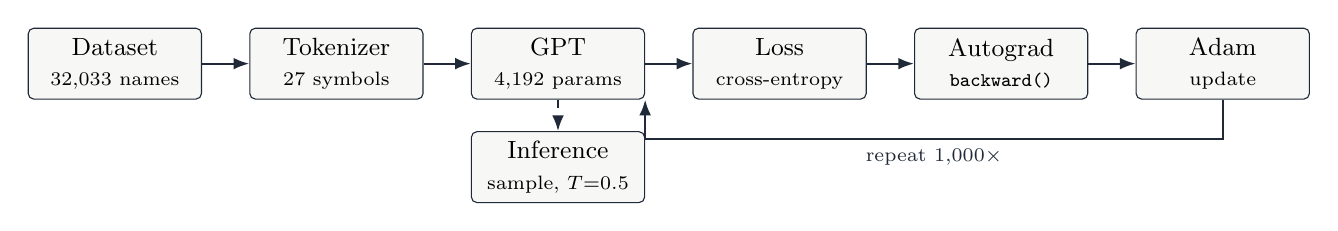
\begin{tikzpicture}[
  node distance=4mm and 6mm,
  box/.style={draw=ink,rounded corners=2pt,fill=codebg,minimum height=9mm,
              minimum width=22mm,align=center,font=\small},
  arr/.style={-{Latex[length=2mm]},thick,ink}]
\node[box] (data) {Dataset\\ \scriptsize 32{,}033 names};
\node[box,right=of data] (tok) {Tokenizer\\ \scriptsize 27 symbols};
\node[box,right=of tok] (model) {GPT\\ \scriptsize 4{,}192 params};
\node[box,right=of model] (loss) {Loss\\ \scriptsize cross-entropy};
\node[box,right=of loss] (grad) {Autograd\\ \scriptsize \texttt{backward()}};
\node[box,right=of grad] (opt) {Adam\\ \scriptsize update};
\node[box,below=of model] (inf) {Inference\\ \scriptsize sample, $T{=}0.5$};
\draw[arr] (data)--(tok); \draw[arr] (tok)--(model); \draw[arr] (model)--(loss);
\draw[arr] (loss)--(grad); \draw[arr] (grad)--(opt);
\draw[arr] (opt.south) |- ++(0,-5mm) -| node[pos=0.25,below,font=\scriptsize]{repeat $1{,}000\times$} (model.south east);
\draw[arr,dashed] (model.south) -- (inf.north);
\end{tikzpicture}
\caption{The microgpt pipeline. Training repeats the forward--loss--backward--update loop once per document. Inference reuses the same model function, feeding each sampled token back in.}
\label{fig:pipeline}
\end{figure}

\subsection{Where to get the code}

\begin{itemize}[leftmargin=2em]
  \item Blog post (the primary text for these notes): \url{https://karpathy.github.io/2026/02/12/microgpt/}
  \item The gist \texttt{microgpt.py}: \url{https://gist.github.com/karpathy/8627fe009c40f57531cb18360106ce95}
  \item The step-by-step build \texttt{build\_microgpt.py}, whose revision history is \texttt{train0.py} through \texttt{train5.py}: \url{https://gist.github.com/karpathy/561ac2de12a47cc06a23691e1be9543a}
  \item A Google Colab notebook \parencite{karpathy2026microgptcolab}, and a one-page web rendering at \url{https://karpathy.ai/microgpt.html}.
\end{itemize}

Run it with \code{python microgpt.py}. There is nothing to install. On a laptop the run takes a minute or two; the timing we measured for these notes is reported in \cref{sec:runit}.

\subsection{Notation}

We write $V$ for the vocabulary size ($V=27$), $d$ for the embedding width ($d=16$, called \code{n_embd} in the code), $H$ for the number of heads ($H=4$), $d_h = d/H$ for the head width ($d_h=4$), $L$ for the number of layers ($L=1$) and $T_{\max}$ for the context length ($T_{\max}=16$, \code{block_size}). Vectors are columns in $\R^d$ unless stated otherwise; a weight matrix $W\in\R^{n_{\text{out}}\times n_{\text{in}}}$ acts by $W x$. This matches the code, where \code{matrix(nout, nin)} builds a list of \code{nout} rows each of length \code{nin}, and \code{linear(x, w)} computes one dot product per row.

% =============================================================================
\section{Dataset: text as a stream of documents}
% =============================================================================

\subsection{The code}

\begin{lstlisting}
# Let there be a Dataset `docs`: list[str] of documents (e.g. a list of names)
if not os.path.exists('input.txt'):
    import urllib.request
    names_url = 'https://raw.githubusercontent.com/karpathy/makemore/988aa59/names.txt'
    urllib.request.urlretrieve(names_url, 'input.txt')
docs = [line.strip() for line in open('input.txt') if line.strip()]
random.shuffle(docs)
print(f"num docs: {len(docs)}")
\end{lstlisting}

The file \texttt{names.txt} comes from the makemore project \parencite{karpathy2022makemore}. It contains 32{,}033 lowercase first names, one per line (\emph{emma, olivia, ava, isabella, \dots}). Each line is treated as one \emph{document}. The longest name has 15 characters, which is why the context length is set to 16 later on.

\subsection{Why ``documents''}

The language-modelling task is to learn the probability distribution of sequences in the training data and then to sample new sequences from it. In production the documents are web pages, books and code \parencite{raffel2020t5,gao2020pile,penedo2024fineweb}; here they are names. Nothing else in the program depends on what the documents contain, which is the point of the FAQ entry ``What if I change the dataset?'': swap in city names or short poems and the remaining 190 lines are unchanged.

\begin{keyidea}[: a conversation is just a document]
From the model's point of view, a ChatGPT conversation is a single, oddly formatted document. The system prompt and the user's message are the prefix; the model's reply is a statistical \emph{completion} of that document, produced one token at a time. microgpt completing \emph{k-a-r} into \emph{karai} and ChatGPT completing a prompt into a paragraph are the same operation.
\end{keyidea}

\subsection{Literature}

Treating text as a sequence to be predicted goes back to \textcite{shannon1948mathematical,shannon1951prediction}, who measured how predictable English letters are and introduced the entropy of a source, which we meet again when we interpret the loss (\cref{sec:loss}). Neural language models in the modern sense begin with \textcite{bengio2003neural}; character-level neural generation of text, the closest ancestor of microgpt's task, was popularised by \textcite{sutskever2011generating}, \textcite{graves2013generating} and Karpathy's own essay on recurrent networks \parencite{karpathy2015rnn}.

% =============================================================================
\section{Tokenizer: characters as discrete symbols}
% =============================================================================

\subsection{The code}

\begin{lstlisting}
# Let there be a Tokenizer to translate strings to sequences of integers ("tokens") and back
uchars = sorted(set(''.join(docs))) # unique characters in the dataset become token ids 0..n-1
BOS = len(uchars) # token id for a special Beginning of Sequence (BOS) token
vocab_size = len(uchars) + 1 # total number of unique tokens, +1 is for BOS
print(f"vocab size: {vocab_size}")
\end{lstlisting}

The unique characters in the names are the 26 lowercase letters, sorted so that \texttt{a}$\mapsto 0$, \dots, \texttt{z}$\mapsto 25$. One extra symbol, \BOS{} (``beginning of sequence''), gets id 26, so $V = 27$. Encoding is \code{uchars.index(ch)}; decoding is \code{uchars[token_id]}.

\subsection{Tokens are symbols, not numbers}

The integer ids carry no arithmetic meaning: 4 is not ``twice'' 2, and \texttt{e} is not between \texttt{d} and \texttt{f} in any sense the model is told about. Karpathy's phrasing is that the ids ``might as well be different emoji''. The first thing the network does with an id is to look up a learned vector for it (\cref{sec:embeddings}), which is where meaning is eventually attached.

\subsection{The role of \BOS}

Every training document is wrapped as \texttt{[BOS, e, m, m, a, BOS]}. The leading \BOS{} gives the model a starting context from which to predict the first letter; the trailing \BOS{} is a target the model must learn to emit when a name is finished. At inference the loop starts by feeding \BOS{} and stops when \BOS{} is sampled. A single symbol therefore plays the roles that other systems split into \texttt{<s>}/\texttt{</s>} or \texttt{<|endoftext|>}.

\subsection{Literature: from characters to byte-pair encoding}

Production tokenizers do not work on single characters. GPT-2 \parencite{radford2019gpt2} and tiktoken \parencite{openai2022tiktoken} use byte-level \emph{byte-pair encoding} (BPE). BPE was invented as a compression algorithm by \textcite{gage1994bpe} and brought to neural machine translation by \textcite{sennrich2016bpe}: starting from bytes, repeatedly merge the most frequent adjacent pair into a new symbol until the vocabulary reaches a target size (around 50k for GPT-2, around 100k for GPT-4). Common words become one token and rare words are split into pieces, so the model sees more content per position and can attend over longer stretches of text. SentencePiece \parencite{kudo2018sentencepiece} is the other widely used implementation. Karpathy's tokenizer lecture \parencite{karpathy2024tokenizervideo} builds a BPE tokenizer from scratch and is the natural next step after these notes.

% =============================================================================
\section{Autograd: the chain rule as a data structure}
\label{sec:autograd}
% =============================================================================

Training adjusts parameters to lower a loss, so for every parameter $\theta$ we need $\partial \mathcal L/\partial\theta$: ``if I nudge this number up a little, does the loss go up or down, and by how much?'' The computation has thousands of inputs and one scalar output, which is exactly the setting in which \emph{reverse-mode} automatic differentiation, better known as backpropagation, is efficient: one backward sweep yields all gradients at a cost comparable to one forward pass.

\subsection{The \texttt{Value} class}

\begin{lstlisting}
class Value:
    __slots__ = ('data', 'grad', '_children', '_local_grads')

    def __init__(self, data, children=(), local_grads=()):
        self.data = data                # scalar value of this node calculated during forward pass
        self.grad = 0                   # derivative of the loss w.r.t. this node, calculated in backward pass
        self._children = children       # children of this node in the computation graph
        self._local_grads = local_grads # local derivative of this node w.r.t. its children

    def __add__(self, other):
        other = other if isinstance(other, Value) else Value(other)
        return Value(self.data + other.data, (self, other), (1, 1))

    def __mul__(self, other):
        other = other if isinstance(other, Value) else Value(other)
        return Value(self.data * other.data, (self, other), (other.data, self.data))

    def __pow__(self, other): return Value(self.data**other, (self,), (other * self.data**(other-1),))
    def log(self): return Value(math.log(self.data), (self,), (1/self.data,))
    def exp(self): return Value(math.exp(self.data), (self,), (math.exp(self.data),))
    def relu(self): return Value(max(0, self.data), (self,), (float(self.data > 0),))
    def __neg__(self): return self * -1
    def __radd__(self, other): return self + other
    def __sub__(self, other): return self + (-other)
    def __rsub__(self, other): return other + (-self)
    def __rmul__(self, other): return self * other
    def __truediv__(self, other): return self * other**-1
    def __rtruediv__(self, other): return other * self**-1
\end{lstlisting}

A \code{Value} wraps one floating-point number and records how it was produced: which nodes it was computed from (\code{_children}) and the derivative of the output with respect to each of them (\code{_local_grads}). Every arithmetic operation returns a fresh node, so a forward computation silently builds a directed acyclic graph (DAG) whose leaves are parameters and constants and whose single root is the loss.

Only six primitive operations are needed; everything else is defined in terms of them (subtraction is addition of a negation, division is multiplication by a power of $-1$).

\begin{table}[h]
\centering\small
\begin{tabular}{@{}lll@{}}
\toprule
Operation & Forward & Local gradients stored \\
\midrule
\code{a + b} & $a+b$ & $\partial/\partial a = 1,\quad \partial/\partial b = 1$ \\
\code{a * b} & $a\cdot b$ & $\partial/\partial a = b,\quad \partial/\partial b = a$ \\
\code{a ** n} & $a^n$ & $\partial/\partial a = n\,a^{\,n-1}$ \\
\code{a.log()} & $\ln a$ & $\partial/\partial a = 1/a$ \\
\code{a.exp()} & $e^a$ & $\partial/\partial a = e^a$ \\
\code{a.relu()} & $\max(0,a)$ & $\partial/\partial a = \mathbf 1[a>0]$ \\
\bottomrule
\end{tabular}
\caption{The six ``lego blocks'' of the autograd engine. Each stores its local derivative at construction time, using the forward values that are available at that moment.}
\label{tab:lego}
\end{table}

\begin{remark}
The local gradient is computed and stored during the \emph{forward} pass, when the operand values are at hand. The backward pass therefore never recomputes anything; it only multiplies and adds stored numbers. This is the design of micrograd \parencite{karpathy2020micrograd} and, conceptually, of PyTorch's autograd \parencite{paszke2017autodiff}.
\end{remark}

\subsection{The backward pass}

\begin{lstlisting}
    def backward(self):
        topo = []
        visited = set()
        def build_topo(v):
            if v not in visited:
                visited.add(v)
                for child in v._children:
                    build_topo(child)
                topo.append(v)
        build_topo(self)
        self.grad = 1
        for v in reversed(topo):
            for child, local_grad in zip(v._children, v._local_grads):
                child.grad += local_grad * v.grad
\end{lstlisting}

Three things happen.

\paragraph{Topological sort.} A depth-first search from the root appends each node to \code{topo} \emph{after} all of its children, so \code{topo} lists nodes from leaves to root. Reversing it gives an order in which every node is visited before anything it depends on; that is exactly what the chain rule needs, because a node's gradient must be final before it is propagated to its children.

\paragraph{Seed.} The loss node receives $\partial\mathcal L/\partial \mathcal L = 1$.

\paragraph{Chain rule with accumulation.} For a node $v$ with child $c$ and stored local gradient $\partial v/\partial c$,
\begin{equation}
\dd{\mathcal L}{c} \mathrel{+}= \dd{v}{c}\cdot\dd{\mathcal L}{v}. \label{eq:chain}
\end{equation}
The \code{+=} is essential. If $c$ feeds into several nodes, the loss depends on $c$ along several paths, and the multivariable chain rule says the total derivative is the \emph{sum} over paths. Karpathy's analogy: a car twice as fast as a bicycle, which is four times as fast as a walker, is $2\times 4 = 8$ times as fast as the walker; rates multiply along a path, and when there are several paths, their contributions add.

\subsection{A worked example}

\begin{lstlisting}
a = Value(2.0)
b = Value(3.0)
c = a * b       # c = 6.0
L = c + a       # L = 8.0
L.backward()
print(a.grad)   # 4.0 (dL/da = b + 1 = 3 + 1, via both paths)
print(b.grad)   # 2.0 (dL/db = a = 2)
\end{lstlisting}

\begin{figure}[h]
\centering
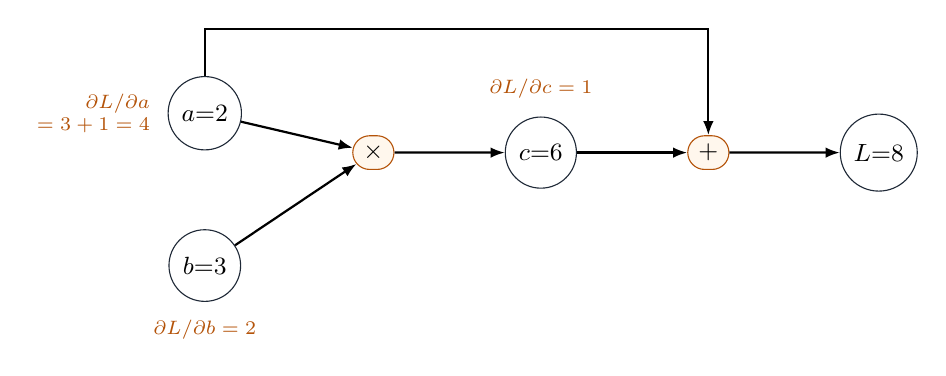
\begin{tikzpicture}[
  node distance=10mm and 14mm,
  v/.style={draw=ink,circle,minimum size=9mm,font=\small,fill=white},
  op/.style={draw=accent,rounded rectangle,fill=boxbg,font=\small,inner sep=3pt},
  arr/.style={-{Latex[length=1.8mm]},thick},
  g/.style={font=\scriptsize,accent}]
\node[v] (a) {$a{=}2$};
\node[v,below=of a] (b) {$b{=}3$};
\node[op,right=of a,yshift=-5mm] (mul) {$\times$};
\node[v,right=of mul] (c) {$c{=}6$};
\node[op,right=of c] (add) {$+$};
\node[v,right=of add] (L) {$L{=}8$};
\draw[arr] (a)--(mul); \draw[arr] (b)--(mul); \draw[arr] (mul)--(c);
\draw[arr] (c)--(add); \draw[arr] (add)--(L);
\draw[arr] (a.north) -- ++(0,6mm) -| (add.north);
\node[g,left=1mm of a,align=right] {$\partial L/\partial a$\\$= 3 + 1 = 4$};
\node[g,below=1mm of b] {$\partial L/\partial b = 2$};
\node[g,above=1mm of c] {$\partial L/\partial c = 1$};
\end{tikzpicture}
\caption{The graph for $L = ab + a$. The node $a$ has two parents ($\times$ and $+$), so its gradient accumulates from both: $b\cdot 1 + 1\cdot 1 = 4$.}
\end{figure}

Interpretation: $a.\mathrm{grad}=4$ means that increasing $a$ by $0.001$ raises $L$ by about $0.004$. The sign gives the direction of influence, the magnitude its steepness. Gradient descent uses exactly this information in reverse: to lower $L$, move each input a little against its gradient.

\subsection{What PyTorch does differently}

The same program in PyTorch gives identical numbers:
\begin{lstlisting}
import torch
a = torch.tensor(2.0, requires_grad=True)
b = torch.tensor(3.0, requires_grad=True)
c = a * b
L = c + a
L.backward()
print(a.grad)   # tensor(4.)
print(b.grad)   # tensor(2.)
\end{lstlisting}
PyTorch's engine \parencite{paszke2019pytorch} runs the same algorithm over \emph{tensors}, so that one node of its graph can stand for millions of scalars and one backward operation can be a fused GPU kernel. microgpt's graph contains one node per scalar operation. Running one training step on the name ``emma'' creates on the order of a hundred thousand \code{Value} objects (we count them in \cref{sec:runit}), which is why the pure-Python version is slow and why nobody trains real models this way. The mathematics, however, is identical.

\subsection{Literature}

Reverse-mode automatic differentiation was published by \textcite{linnainmaa1976taylor}; its application to neural networks under the name backpropagation is due to \textcite{rumelhart1986learning}. \textcite{griewank2008evaluating} is the standard mathematical treatment, and \textcite{baydin2018autodiff} survey the field for a machine-learning audience, including the distinction between forward and reverse mode and the role of the computational graph. Karpathy's 2.5-hour micrograd lecture \parencite{karpathy2022microgradvideo} builds the \code{Value} class line by line.

% =============================================================================
\section{Parameters: the knowledge of the model}
\label{sec:params}
% =============================================================================

\begin{lstlisting}
n_layer = 1     # depth of the transformer neural network (number of layers)
n_embd = 16     # width of the network (embedding dimension)
block_size = 16 # maximum context length of the attention window (note: the longest name is 15 characters)
n_head = 4      # number of attention heads
head_dim = n_embd // n_head # derived dimension of each head
matrix = lambda nout, nin, std=0.08: [[Value(random.gauss(0, std)) for _ in range(nin)] for _ in range(nout)]
state_dict = {'wte': matrix(vocab_size, n_embd), 'wpe': matrix(block_size, n_embd), 'lm_head': matrix(vocab_size, n_embd)}
for i in range(n_layer):
    state_dict[f'layer{i}.attn_wq'] = matrix(n_embd, n_embd)
    state_dict[f'layer{i}.attn_wk'] = matrix(n_embd, n_embd)
    state_dict[f'layer{i}.attn_wv'] = matrix(n_embd, n_embd)
    state_dict[f'layer{i}.attn_wo'] = matrix(n_embd, n_embd)
    state_dict[f'layer{i}.mlp_fc1'] = matrix(4 * n_embd, n_embd)
    state_dict[f'layer{i}.mlp_fc2'] = matrix(n_embd, 4 * n_embd)
params = [p for mat in state_dict.values() for row in mat for p in row]
print(f"num params: {len(params)}")
\end{lstlisting}

Every parameter is a \code{Value} initialised from $\mathcal N(0,\,0.08^2)$. The dictionary \code{state_dict} borrows PyTorch's name and organises the parameters into matrices; \code{params} flattens them into one list so that the optimizer can loop over them.

\subsection{Counting the parameters}

\begin{table}[h]
\centering\small
\begin{tabular}{@{}llrr@{}}
\toprule
Name & Shape & Formula & Count \\
\midrule
\code{wte} & $V\times d$ & $27\times 16$ & 432 \\
\code{wpe} & $T_{\max}\times d$ & $16\times 16$ & 256 \\
\code{lm_head} & $V\times d$ & $27\times 16$ & 432 \\
\code{attn_wq, attn_wk, attn_wv, attn_wo} & $4\times(d\times d)$ & $4\times 16\times 16$ & 1{,}024 \\
\code{mlp_fc1} & $4d\times d$ & $64\times 16$ & 1{,}024 \\
\code{mlp_fc2} & $d\times 4d$ & $16\times 64$ & 1{,}024 \\
\midrule
Total & & & \textbf{4{,}192} \\
\bottomrule
\end{tabular}
\caption{Parameter inventory for the default configuration ($L=1$). Per layer, the Transformer block holds $12d^2 = 3{,}072$ parameters, split evenly between attention ($4d^2$) and the MLP ($8d^2$).}
\label{tab:params}
\end{table}

For comparison: GPT-2 \parencite{radford2019gpt2} has 1.5 billion parameters in its largest configuration (Karpathy quotes 1.6B), GPT-3 has 175 billion \parencite{brown2020gpt3}, and current frontier models have hundreds of billions to trillions. The $12 d^2$ per-layer rule generalises: for $d = 1600$ and 48 layers, the GPT-2 XL block parameters come to $48\times 12\times 1600^2 \approx 1.47$B.

\subsection{Why these initialisation choices}

\begin{itemize}[leftmargin=2em]
  \item \textbf{Small Gaussian.} Weights must be random so that different neurons compute different things (symmetry breaking), and small so that early activations and softmaxes are not saturated. The scale $0.08$ is close to $1/\sqrt{d}=0.25$ divided by about three; the classical analysis of why the scale should shrink with fan-in is \textcite{glorot2010init}. GPT-2 used $0.02$ with $d\ge 768$.
  \item \textbf{No biases.} Modern LLMs (LLaMA and successors, \citeauthor{touvron2023llama} \citeyear{touvron2023llama}) drop bias vectors; they add parameters without measurable benefit once normalisation layers are present.
  \item \textbf{No weight tying.} GPT-2 shares \code{wte} with \code{lm_head} \parencite{press2017weighttying}; microgpt keeps them separate, which is simpler to read and costs only 432 extra parameters here.
\end{itemize}

% =============================================================================
\section{Architecture: a GPT-2-style Transformer, one token at a time}
\label{sec:arch}
% =============================================================================

The model is a \emph{stateless function}: given a token id, its position, the parameters, and the keys and values cached from earlier positions, it returns $V$ logits, one score per possible next token. Karpathy follows GPT-2 \parencite{radford2019gpt2} with three simplifications, announced in a comment in the source:
\begin{center}
\emph{layernorm $\to$ rmsnorm, \quad no biases, \quad GeLU $\to$ ReLU.}
\end{center}

\subsection{Three helpers}

\begin{lstlisting}
def linear(x, w):
    return [sum(wi * xi for wi, xi in zip(wo, x)) for wo in w]

def softmax(logits):
    max_val = max(val.data for val in logits)
    exps = [(val - max_val).exp() for val in logits]
    total = sum(exps)
    return [e / total for e in exps]

def rmsnorm(x):
    ms = sum(xi * xi for xi in x) / len(x)
    scale = (ms + 1e-5) ** -0.5
    return [xi * scale for xi in x]
\end{lstlisting}

\paragraph{\code{linear}} is a matrix--vector product $y = Wx$, one dot product per row of $W$. It is the only place where parameters touch activations (apart from the embedding lookups), so every learned transformation in the network is linear, and all non-linearity comes from softmax, ReLU and normalisation.

\paragraph{\code{softmax}} turns a vector of real scores $z\in\R^n$ into a probability vector,
\begin{equation}
\softmax(z)_i = \frac{e^{z_i}}{\sum_j e^{z_j}} = \frac{e^{z_i - m}}{\sum_j e^{z_j - m}}\quad\text{for any constant } m.
\end{equation}
Subtracting $m=\max_j z_j$ changes nothing mathematically but keeps every exponent $\le 0$, so \code{exp} cannot overflow. Note that \code{max_val} is a plain float read from \code{.data}; the subtraction is therefore a constant shift in the graph and does not need its own gradient. (Its gradient would cancel exactly anyway.)

\paragraph{\code{rmsnorm}} \parencite{zhang2019rmsnorm} rescales a vector to unit root-mean-square:
\begin{equation}
\rmsnorm(x) = \frac{x}{\sqrt{\tfrac1d\sum_i x_i^2 + \varepsilon}},\qquad \varepsilon = 10^{-5}.
\end{equation}
Compared with LayerNorm \parencite{ba2016layernorm} it drops the mean subtraction and, in microgpt, the learned per-dimension gain as well. Its job is to keep activation magnitudes from drifting as signals flow through the network, which stabilises optimisation.

\subsection{The model function}

\begin{lstlisting}
def gpt(token_id, pos_id, keys, values):
    tok_emb = state_dict['wte'][token_id] # token embedding
    pos_emb = state_dict['wpe'][pos_id] # position embedding
    x = [t + p for t, p in zip(tok_emb, pos_emb)] # joint token and position embedding
    x = rmsnorm(x) # note: not redundant due to backward pass via the residual connection

    for li in range(n_layer):
        # 1) Multi-head Attention block
        x_residual = x
        x = rmsnorm(x)
        q = linear(x, state_dict[f'layer{li}.attn_wq'])
        k = linear(x, state_dict[f'layer{li}.attn_wk'])
        v = linear(x, state_dict[f'layer{li}.attn_wv'])
        keys[li].append(k)
        values[li].append(v)
        x_attn = []
        for h in range(n_head):
            hs = h * head_dim
            q_h = q[hs:hs+head_dim]
            k_h = [ki[hs:hs+head_dim] for ki in keys[li]]
            v_h = [vi[hs:hs+head_dim] for vi in values[li]]
            attn_logits = [sum(q_h[j] * k_h[t][j] for j in range(head_dim)) / head_dim**0.5 for t in range(len(k_h))]
            attn_weights = softmax(attn_logits)
            head_out = [sum(attn_weights[t] * v_h[t][j] for t in range(len(v_h))) for j in range(head_dim)]
            x_attn.extend(head_out)
        x = linear(x_attn, state_dict[f'layer{li}.attn_wo'])
        x = [a + b for a, b in zip(x, x_residual)]
        # 2) MLP block
        x_residual = x
        x = rmsnorm(x)
        x = linear(x, state_dict[f'layer{li}.mlp_fc1'])
        x = [xi.relu() for xi in x]
        x = linear(x, state_dict[f'layer{li}.mlp_fc2'])
        x = [a + b for a, b in zip(x, x_residual)]

    logits = linear(x, state_dict['lm_head'])
    return logits
\end{lstlisting}

\begin{figure}[p]
\centering
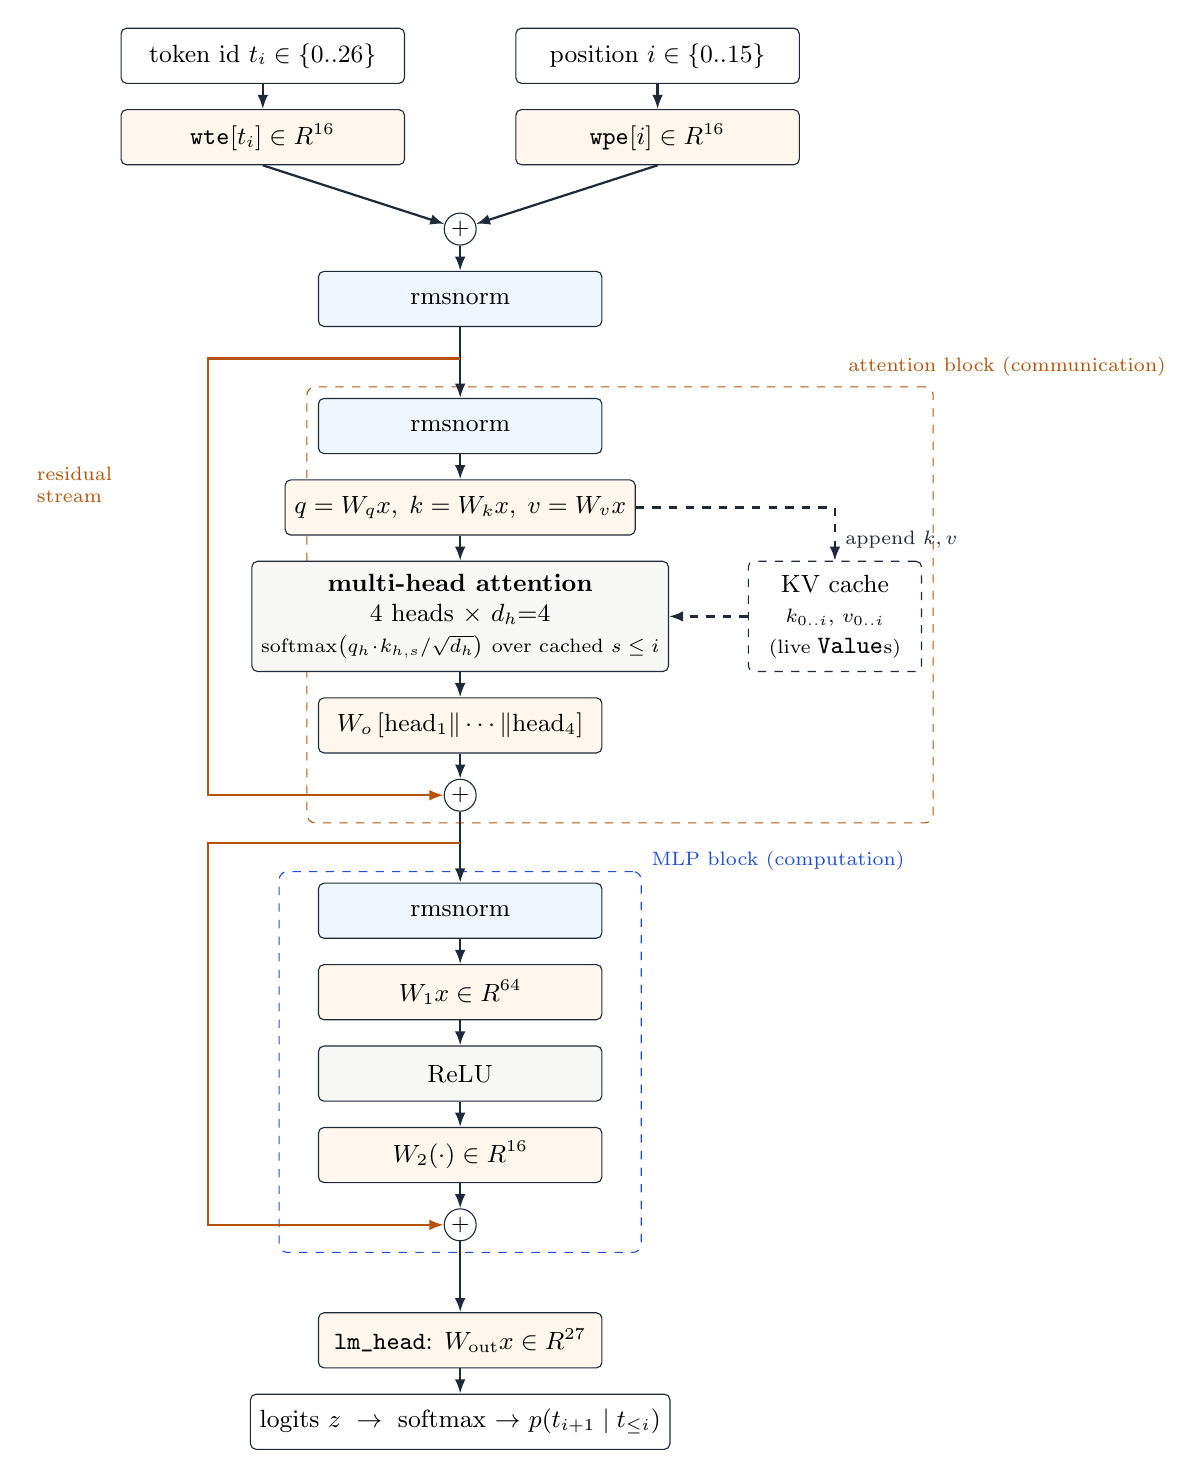
\begin{tikzpicture}[
  font=\small,
  node distance=3.2mm,
  blk/.style={draw=ink,rounded corners=2pt,fill=codebg,minimum width=36mm,minimum height=7mm,align=center},
  prm/.style={blk,fill=boxbg},
  nrm/.style={blk,fill=boxbg2},
  add/.style={draw=ink,circle,inner sep=1pt,fill=white,font=\footnotesize},
  arr/.style={-{Latex[length=1.8mm]},thick,ink},
  lbl/.style={font=\scriptsize,ink,anchor=west,align=left}]
% inputs
\node[blk,fill=white] (tok) {token id $t_i\in\{0..26\}$};
\node[blk,fill=white,right=14mm of tok] (pos) {position $i\in\{0..15\}$};
\node[prm,below=of tok] (wte) {\code{wte}$[t_i]\in\R^{16}$};
\node[prm,below=of pos] (wpe) {\code{wpe}$[i]\in\R^{16}$};
\node[add,below=6mm of $(wte.south)!0.5!(wpe.south)$] (add0) {$+$};
\node[nrm,below=of add0] (n0) {rmsnorm};
% attention block
\node[nrm,below=9mm of n0] (n1) {rmsnorm};
\node[prm,below=of n1] (qkv) {$q=W_q x,\; k=W_k x,\; v=W_v x$};
\node[blk,below=of qkv,minimum height=14mm] (attn) {\textbf{multi-head attention}\\ 4 heads $\times$ $d_h{=}4$\\ \scriptsize softmax$\big(q_h\!\cdot\! k_{h,s}/\sqrt{d_h}\big)$ over cached $s\le i$};
\node[prm,below=of attn] (wo) {$W_o\,[\text{head}_1\|\cdots\|\text{head}_4]$};
\node[add,below=of wo] (add1) {$+$};
% KV cache
\node[blk,fill=white,dashed,right=10mm of attn,minimum width=22mm,minimum height=14mm] (kv) {KV cache\\ \scriptsize $k_{0..i},\,v_{0..i}$\\ \scriptsize (live \code{Value}s)};
\draw[arr,dashed] (qkv.east) -| node[pos=0.8,right,font=\scriptsize]{append $k,v$} (kv.north);
\draw[arr,dashed] (kv.west) -- (attn.east);
% MLP block
\node[nrm,below=9mm of add1] (n2) {rmsnorm};
\node[prm,below=of n2] (fc1) {$W_1 x\in\R^{64}$};
\node[blk,below=of fc1] (relu) {ReLU};
\node[prm,below=of relu] (fc2) {$W_2(\cdot)\in\R^{16}$};
\node[add,below=of fc2] (add2) {$+$};
% head
\node[prm,below=9mm of add2] (lm) {\code{lm_head}: $W_{\text{out}}x\in\R^{27}$};
\node[blk,fill=white,below=of lm] (logits) {logits $z$ \;$\to$\; softmax $\to$ $p(t_{i+1}\mid t_{\le i})$};
% arrows main
\draw[arr] (tok)--(wte); \draw[arr] (pos)--(wpe);
\draw[arr] (wte.south)--(add0); \draw[arr] (wpe.south)--(add0);
\draw[arr] (add0)--(n0); \draw[arr] (n0)--(n1); \draw[arr] (n1)--(qkv); \draw[arr] (qkv)--(attn);
\draw[arr] (attn)--(wo); \draw[arr] (wo)--(add1); \draw[arr] (add1)--(n2); \draw[arr] (n2)--(fc1);
\draw[arr] (fc1)--(relu); \draw[arr] (relu)--(fc2); \draw[arr] (fc2)--(add2); \draw[arr] (add2)--(lm); \draw[arr] (lm)--(logits);
% residuals
\draw[arr,accent] ($(n0.south)+(0,-4mm)$) -- ++(-32mm,0) |- (add1.west);
\draw[arr,accent] ($(add1.south)+(0,-4mm)$) -- ++(-32mm,0) |- (add2.west);
\node[lbl,accent] at ($(n0.south)+(-55mm,-20mm)$) {residual\\ stream};
% block brace
\begin{scope}[on background layer]
\node[draw=accent,dashed,rounded corners=3pt,fit=(n1)(add1)(kv),inner sep=4pt,label={[accent,font=\scriptsize]above right:attention block (communication)}] {};
\node[draw=accent2,dashed,rounded corners=3pt,fit=(n2)(add2),inner xsep=14pt,inner ysep=4pt,label={[accent2,font=\scriptsize]above right:MLP block (computation)}] {};
\end{scope}
\end{tikzpicture}
\caption{One call of \code{gpt(token_id, pos_id, keys, values)} for $L=1$. Orange boxes hold parameters, blue boxes are parameter-free normalisations. The two orange side-arrows are the residual connections. With $L>1$ the dashed region repeats $L$ times; the KV cache has one list of keys and one of values per layer.}
\label{fig:arch}
\end{figure}

\subsection{Embeddings}
\label{sec:embeddings}

A network cannot do arithmetic on the symbol ``5''. Each token id selects a learned row of the table \code{wte} $\in\R^{V\times d}$, and each position selects a row of \code{wpe} $\in\R^{T_{\max}\times d}$. The two vectors are added:
\begin{equation}
x^{(0)}_i = \rmsnorm\big(\mathrm{wte}[t_i] + \mathrm{wpe}[i]\big).
\end{equation}
The result encodes \emph{what} the token is and \emph{where} it is. Because the rest of the network is permutation-invariant in the cached positions (attention is a weighted sum), the position embedding is the only source of order information. The original Transformer used fixed sinusoids \parencite{vaswani2017attention}; GPT-1 and GPT-2 learned the table as here \parencite{radford2018gpt1,radford2019gpt2}; most current models use rotary embeddings (RoPE, \citeauthor{su2021rope} \citeyear{su2021rope}) which inject \emph{relative} position into $q$ and $k$ instead.

\begin{remark}[On the first \code{rmsnorm}]
The source comments that normalising the embedding sum is ``not redundant due to backward pass via the residual connection''. The pre-norm inside the attention block only normalises the copy of $x$ that enters the branch; the copy that continues down the residual path is untouched. Normalising once at the start therefore fixes the scale at which the residual stream begins, which matters for both the forward values and the gradients that flow back along the stream.
\end{remark}

\subsection{Attention}
\label{sec:attention}

The current normalised vector $x$ is projected into a query, a key and a value:
\begin{equation}
q = W_q x,\qquad k = W_k x,\qquad v = W_v x,\qquad W_q,W_k,W_v\in\R^{d\times d}.
\end{equation}
Karpathy's gloss: the query asks ``what am I looking for?'', the key says ``what do I contain?'', the value says ``what do I offer if selected?''. The new $k$ and $v$ are appended to the per-layer cache, so after processing positions $0,\dots,i$ the cache holds $k_0,\dots,k_i$ and $v_0,\dots,v_i$.

Each of the $H$ heads works on its own slice of the $d$ coordinates. For head $h$ with slice $S_h = \{h d_h,\dots,(h+1)d_h-1\}$:
\begin{align}
a_{h,s} &= \frac{q[S_h]\cdot k_s[S_h]}{\sqrt{d_h}},\qquad s=0,\dots,i, \label{eq:attnlogit}\\
\alpha_{h} &= \softmax(a_{h,0},\dots,a_{h,i}), \label{eq:attnw}\\
\mathrm{head}_h &= \sum_{s=0}^{i}\alpha_{h,s}\, v_s[S_h]\in\R^{d_h}. \label{eq:headout}
\end{align}
The head outputs are concatenated into a vector of length $d$ and projected by $W_o$. In matrix form this is the familiar
\begin{equation}
\operatorname{Attention}(Q,K,V) = \softmax\!\Big(\frac{QK^{\top}}{\sqrt{d_h}}\Big)V
\end{equation}
of \textcite{vaswani2017attention}, specialised to a single query row.

\paragraph{Where is the causal mask?} Vectorised implementations compute all $T\times T$ scores at once and then mask out $s>i$ with $-\infty$. microgpt needs no mask: at position $i$ the cache simply does not yet contain anything from the future. Causality is a consequence of processing tokens in order.

\paragraph{Why $\sqrt{d_h}$?} If $q$ and $k$ have independent coordinates of unit variance, their dot product has variance $d_h$. Dividing by $\sqrt{d_h}$ restores unit variance, so the softmax is neither flat nor saturated at initialisation \parencite{vaswani2017attention}. With $d_h=4$ the factor is $1/2$.

\paragraph{Why several heads?} Each head has its own $W_q,W_k,W_v$ slices and so can implement a different pattern of lookup (``the previous letter'', ``the most recent vowel'', ``the first letter of the name''). Four heads of width four cost exactly the same as one head of width sixteen; the split buys diversity, not capacity.

\begin{keyidea}[: attention is communication]
The attention block is the \emph{only} place where position $i$ reads information from positions $0,\dots,i-1$. Everything else in the network acts on one position at a time. Karpathy's summary: the Transformer interleaves \emph{communication} (attention) with \emph{computation} (MLP), both wired into a shared residual stream.
\end{keyidea}

\subsection{The KV cache, during training}

Readers who know Transformers from the serving side associate the KV cache with inference. microgpt uses it during training too, and the post argues that the cache is ``conceptually always there'': a batched implementation computes all keys and values for a sequence in one matrix multiply and the cache is simply hidden inside that tensor. Because microgpt processes one token at a time, the cache becomes explicit.

The subtle point is that the cached entries are \emph{live} \code{Value} nodes. When the loss at position 7 depends on $k_2$ and $v_2$, the backward pass flows gradient into the parameters that produced them, through the cache. In production inference the cached tensors are detached; in production training there is no explicit cache but the same gradient paths exist inside the attention kernel. The memory cost of the cache, $2\,L\,T\,d$ numbers per sequence, is what motivates multi-query and grouped-query attention \parencite{shazeer2019mqa,ainslie2023gqa} and paged cache management in vLLM \parencite{kwon2023vllm}; \textcite{pope2022efficiently} give the accounting.

\subsection{The MLP block}

\begin{equation}
\mathrm{MLP}(x) = W_2\,\relu(W_1 x),\qquad W_1\in\R^{4d\times d},\; W_2\in\R^{d\times 4d}.
\end{equation}
Project up by a factor of four, apply an elementwise non-linearity, project back down. The $4\times$ widening comes from the original Transformer and GPT-2. The MLP is where per-position ``thinking'' happens: having gathered context through attention, each position transforms its own vector without reference to any other.

GPT-2 used GELU \parencite{hendrycks2016gelu}; microgpt uses ReLU \parencite{nair2010relu,glorot2011relu} because its gradient is a single comparison. Current models mostly use gated variants such as SwiGLU \parencite{shazeer2020glu,touvron2023llama}; squared ReLU \parencite{so2021primer} is another popular simplification used in nanochat \parencite{karpathy2025nanochat}.

\subsection{Residual connections and pre-normalisation}

Both blocks add their output to their input: $x \leftarrow x + f(\rmsnorm(x))$. The identity path means that gradients reach early layers undiminished, which is what makes 100-layer networks trainable \parencite{he2016resnet}. Placing the normalisation \emph{before} each block (pre-LN) rather than after it, as GPT-2 did, makes training markedly more stable \parencite{xiong2020prelayernorm}. The residual-stream picture, in which blocks \emph{read from} and \emph{write to} a shared vector, is developed in \textcite{elhage2021mathematical}.

\subsection{Output}

Finally \code{lm_head} maps the hidden state to $V=27$ logits. Higher logit means the model considers that token more likely to come next. The logits are not probabilities; the softmax that converts them is applied by the caller, inside the loss during training and inside the sampler at inference.

\subsection{Cost of one token}

Counting multiply--adds per position for $L=1$: $4d^2$ for the attention projections, $8d^2$ for the MLP, $Vd$ for the head, plus about $2(i{+}1)d$ for the attention scores and weighted sum at position $i$. For $d=16$ this is about $3{,}500$ multiply--adds, essentially $2\times$ the number of non-embedding parameters. The rule of thumb ``$\approx 2N$ FLOPs per token for a forward pass and $\approx 6N$ for a training step'' \parencite{kaplan2020scaling} already holds for microgpt.

% =============================================================================
\section{Training loop: loss, gradients and Adam}
\label{sec:training}
% =============================================================================

\begin{lstlisting}
# Let there be Adam, the blessed optimizer and its buffers
learning_rate, beta1, beta2, eps_adam = 0.01, 0.85, 0.99, 1e-8
m = [0.0] * len(params) # first moment buffer
v = [0.0] * len(params) # second moment buffer

# Repeat in sequence
num_steps = 1000 # number of training steps
for step in range(num_steps):

    # Take single document, tokenize it, surround it with BOS special token on both sides
    doc = docs[step % len(docs)]
    tokens = [BOS] + [uchars.index(ch) for ch in doc] + [BOS]
    n = min(block_size, len(tokens) - 1)

    # Forward the token sequence through the model, building up the computation graph all the way to the loss
    keys, values = [[] for _ in range(n_layer)], [[] for _ in range(n_layer)]
    losses = []
    for pos_id in range(n):
        token_id, target_id = tokens[pos_id], tokens[pos_id + 1]
        logits = gpt(token_id, pos_id, keys, values)
        probs = softmax(logits)
        loss_t = -probs[target_id].log()
        losses.append(loss_t)
    loss = (1 / n) * sum(losses) # final average loss over the document sequence. May yours be low.

    # Backward the loss, calculating the gradients with respect to all model parameters
    loss.backward()

    # Adam optimizer update: update the model parameters based on the corresponding gradients
    lr_t = learning_rate * (1 - step / num_steps) # linear learning rate decay
    for i, p in enumerate(params):
        m[i] = beta1 * m[i] + (1 - beta1) * p.grad
        v[i] = beta2 * v[i] + (1 - beta2) * p.grad ** 2
        m_hat = m[i] / (1 - beta1 ** (step + 1))
        v_hat = v[i] / (1 - beta2 ** (step + 1))
        p.data -= lr_t * m_hat / (v_hat ** 0.5 + eps_adam)
        p.grad = 0

    print(f"step {step+1:4d} / {num_steps:4d} | loss {loss.data:.4f}", end='\r')
\end{lstlisting}

Each step performs five actions: pick a document, run the model forward over it, compute a loss, backpropagate, update.

\subsection{Next-token prediction}

The document ``emma'' becomes \texttt{[BOS, e, m, m, a, BOS]}, a sequence $t_0,\dots,t_5$. Position $i$ sees token $t_i$ (and, through the cache, everything before it) and must predict $t_{i+1}$. There are $n = \min(T_{\max}, |\text{tokens}|-1)$ such prediction problems per document; for ``emma'' $n=5$. Because the longest name has 15 letters, the clamp to $T_{\max}=16$ never truncates a name.

\subsection{Cross-entropy loss}
\label{sec:loss}

At position $i$ the model's softmax output is a distribution $p(\cdot\mid t_{\le i})$ over the 27 tokens, and the loss is the negative log-probability of the token that actually came next:
\begin{equation}
\ell_i = -\log p(t_{i+1}\mid t_{\le i}),\qquad \mathcal L = \frac1n\sum_{i=0}^{n-1}\ell_i.
\end{equation}

\begin{sidebar}{Why negative log probability?}
Three equivalent views.
\begin{itemize}[leftmargin=1.5em]
  \item \textbf{Surprise.} $-\log p$ is 0 when the model was certain and right, and grows without bound as the probability assigned to the truth shrinks. It is the ``surprisal'' of information theory \parencite{shannon1948mathematical,cover2006elements}.
  \item \textbf{Maximum likelihood.} Minimising $\sum_i -\log p(t_{i+1}\mid t_{\le i})$ over a corpus is maximising the log-likelihood of the corpus under the model, since $\log p(\text{document}) = \sum_i \log p(t_{i+1}\mid t_{\le i})$ by the chain rule of probability.
  \item \textbf{Cross-entropy.} With the one-hot target distribution $y$, $-\sum_k y_k\log p_k = -\log p_{\text{target}}$ is the cross-entropy $H(y,p)$, which exceeds the entropy of the data by exactly the KL divergence from data to model \parencite{goodfellow2016deep,bishop2006prml}.
\end{itemize}
\end{sidebar}

\paragraph{Reference values.} A model that knows nothing assigns $p = 1/27$ to everything, giving
\begin{equation}
\mathcal L_{\text{uniform}} = -\log\tfrac{1}{27} = \ln 27 \approx 3.296 .
\end{equation}
The first printed loss, $3.366$, is close to this; the random initial weights make it slightly worse than uniform. The lowest possible loss is $0$. After 1{,}000 steps the smoothed loss is about $2.3$ (\cref{fig:loss}); Karpathy quotes $\approx 2.37$. Two natural rescalings: the \emph{perplexity} $e^{\mathcal L}$ falls from $27$ to about $10$, meaning the model is as uncertain as if choosing uniformly among ten letters; and $\mathcal L/\ln 2$ gives bits per character, about $3.4$ at the end versus $4.75$ for a uniform guess.

\paragraph{The gradient at the logits.} For completeness, the combined softmax--cross-entropy gradient is remarkably simple:
\begin{equation}
\dd{\ell}{z_k} = p_k - y_k,
\end{equation}
that is, ``predicted probability minus one-hot target''. microgpt never writes this down; the autograd engine derives it from the \code{exp}, \code{log}, division and sum nodes in \cref{tab:lego}. \Cref{sec:exercises} asks you to verify the identity numerically.

\subsection{Batch size one, and what it means for the loss curve}

Each step uses exactly one document. In the language of \textcite{robbins1951stochastic} this is stochastic gradient descent with a minibatch of one sequence (of up to 16 tokens). Two consequences:

\begin{itemize}[leftmargin=2em]
  \item The printed loss is noisy. A step on a short, common name such as ``ann'' yields a lower loss than a step on ``christopher'', regardless of learning. \Cref{fig:loss} shows raw and smoothed curves from our run; the last single-document loss was $2.65$ while the trailing 50-step mean was $2.32$.
  \item The model sees only the first $1{,}000$ of the $32{,}033$ shuffled names, about 3\% of one epoch. Every training document is new, so the training loss is effectively a held-out loss. There is no overfitting to speak of, and no need for a validation split at this scale.
\end{itemize}

\begin{figure}[t]
\centering
\begin{tikzpicture}
\begin{axis}[width=0.9\textwidth,height=6.5cm,
  xlabel={training step},ylabel={loss (nats per token)},
  xmin=0,xmax=1000,ymin=1.4,ymax=3.8,
  grid=major,grid style={codeframe!60},
  legend pos=south west,legend style={font=\small,draw=none,fill=white,fill opacity=0.85,text opacity=1},
  tick label style={font=\small},label style={font=\small}]
\addplot[codeframe!90!ink,only marks,mark=*,mark size=0.5pt,opacity=0.6] table[col sep=comma,x=step,y=loss]{loss.csv};
\addlegendentry{per-document loss}
\addplot[accent,very thick] table[col sep=comma,x=step,y=avg]{loss.csv};
\addlegendentry{trailing 50-step mean}
\addplot[accent2,dashed,thick,domain=0:1000] {ln(27)};
\addlegendentry{$\ln 27\approx 3.30$ (uniform guess)}
\end{axis}
\end{tikzpicture}
\caption{Loss over the 1{,}000 training steps of \texttt{microgpt.py} with the default seed. Each grey dot is one document; the orange line is a trailing average. The spread of the dots is the noise of batch size one, not instability.}
\label{fig:loss}
\end{figure}

\subsection{Backward}

One call to \code{loss.backward()} runs the algorithm of \cref{sec:autograd} over the whole graph, from the loss through the averaging, the per-position softmaxes and the model, including the cached keys and values of earlier positions, down into every parameter. Afterwards each parameter's \code{.grad} is $\partial\mathcal L/\partial\theta$. In our measurements a step on a 12-letter name builds a graph of about $10^5$ nodes; forward takes a quarter of a second and backward a tenth.

\subsection{Adam}

Plain gradient descent would update $\theta \leftarrow \theta - \eta\,g$ with $g = \partial\mathcal L/\partial\theta$. Adam \parencite{kingma2015adam} keeps two exponential moving averages per parameter and uses their ratio:
\begin{align}
m_t &= \beta_1 m_{t-1} + (1-\beta_1)\, g_t, &\hat m_t &= \frac{m_t}{1-\beta_1^{\,t}}, \\
v_t &= \beta_2 v_{t-1} + (1-\beta_2)\, g_t^2, &\hat v_t &= \frac{v_t}{1-\beta_2^{\,t}}, \\
\theta_t &= \theta_{t-1} - \eta_t\,\frac{\hat m_t}{\sqrt{\hat v_t}+\epsilon}.
\end{align}

\begin{itemize}[leftmargin=2em]
  \item $m$ is \textbf{momentum} \parencite{polyak1964momentum}: a running mean of gradients that smooths out the step-to-step noise of single documents, ``like a rolling ball''.
  \item $v$ is a running mean of squared gradients, the idea of RMSProp \parencite{tieleman2012rmsprop}. Dividing by $\sqrt{\hat v}$ gives every parameter its own effective learning rate: parameters whose gradients are consistently large take smaller steps, rarely-updated parameters (such as embedding rows of rare letters) take larger ones.
  \item $\hat m,\hat v$ are \textbf{bias corrections}. Both buffers start at zero and are therefore biased toward zero during the first few dozen steps; dividing by $1-\beta^{t}$ undoes this exactly in expectation.
  \item $\epsilon=10^{-8}$ prevents division by zero.
\end{itemize}

microgpt uses $\beta_1=0.85$, $\beta_2=0.99$ rather than the paper's defaults $0.9$, $0.999$: shorter memories suit a run of only 1{,}000 noisy steps. The learning rate $\eta_t = 0.01\,(1 - t/1000)$ decays linearly to zero, a simple instance of the schedules surveyed by \textcite{loshchilov2017sgdr}; large models typically use a warmup followed by cosine or linear decay. Weight decay \parencite{loshchilov2019adamw}, universal at scale, is omitted here.

After the update every gradient is reset to zero. Without this, the next step's \code{+=} accumulation would add new gradients on top of stale ones.

% =============================================================================
\section{Inference: sampling new names}
\label{sec:inference}
% =============================================================================

\begin{lstlisting}
# Inference: may the model babble back to us
temperature = 0.5 # in (0, 1], control the "creativity" of generated text, low to high
print("\n--- inference (new, hallucinated names) ---")
for sample_idx in range(20):
    keys, values = [[] for _ in range(n_layer)], [[] for _ in range(n_layer)]
    token_id = BOS
    sample = []
    for pos_id in range(block_size):
        logits = gpt(token_id, pos_id, keys, values)
        probs = softmax([l / temperature for l in logits])
        token_id = random.choices(range(vocab_size), weights=[p.data for p in probs])[0]
        if token_id == BOS:
            break
        sample.append(uchars[token_id])
    print(f"sample {sample_idx+1:2d}: {''.join(sample)}")
\end{lstlisting}

With parameters frozen, generation is the same forward function in a loop. Start with an empty cache and the \BOS{} token; compute logits; convert to probabilities; draw one token at random according to those probabilities; feed it back as the next input; stop when \BOS{} is drawn or after $T_{\max}$ tokens. This is \emph{autoregressive} or \emph{ancestral} sampling: the model's own output becomes its input.

\subsection{Temperature}

Dividing the logits by $T$ before the softmax gives
\begin{equation}
p_k^{(T)} = \frac{e^{z_k/T}}{\sum_j e^{z_j/T}}.
\end{equation}
$T=1$ samples from the learned distribution. $T<1$ sharpens it: the ratio between the top two probabilities is raised to the power $1/T$, so the model becomes more conservative. As $T\to 0$ the softmax becomes a one-hot on the arg-max, which is greedy decoding. $T>1$ flattens the distribution toward uniform and produces more varied but less coherent output. The name and formula come from the Boltzmann distribution of statistical physics by way of \textcite{ackley1985boltzmann}; \textcite{hinton2015distilling} discuss it in the modern setting. Truncation methods such as top-$k$ \parencite{fan2018hierarchical} and nucleus sampling \parencite{holtzman2020nucleus} are the usual companions of temperature in production and are a one-line addition here (\cref{sec:exercises}).

\subsection{What the samples show}

With the default seed the twenty samples are \emph{kamon, ann, karai, jaire, vialan, karia, yeran, anna, areli, kaina, konna, keylen, liole, alerin, earan, lenne, kana, lara, alela, anton}. They are pronounceable, alternate consonants and vowels, end at plausible lengths, and a few (\emph{ann}, \emph{anna}, \emph{lara}, \emph{anton}) are real names the model has rediscovered rather than copied; most are not in the training set at all. This is the whole phenomenon of ``hallucination'': the model produces statistically plausible sequences with no notion of whether they are real.

% =============================================================================
\section{Running it}
\label{sec:runit}
% =============================================================================

\begin{lstlisting}[language=bash]
python microgpt.py
\end{lstlisting}

Expected output (the loss line is overwritten in place in the gist version; the blog shows every step):
\begin{lstlisting}[language={}]
num docs: 32033
vocab size: 27
num params: 4192
step    1 / 1000 | loss 3.3660
step    2 / 1000 | loss 3.4243
step    3 / 1000 | loss 3.1778
...
step 1000 / 1000 | loss 2.6497

--- inference (new, hallucinated names) ---
sample  1: kamon
sample  2: ann
sample  3: karai
...
\end{lstlisting}

\paragraph{Measurements for these notes.} Running the unmodified gist on a 2026 laptop with CPython took 3 minutes 24 seconds (Karpathy reports about one minute on his machine). Instrumenting the \code{Value} constructor gives the graph sizes in \cref{tab:nodes}: roughly $8{,}000$ nodes per token, dominated by the $16\times 16$ and $16\times 64$ linear layers, each of which creates one multiplication and one addition node per weight.

\begin{table}[h]
\centering\small
\begin{tabular}{@{}lrrrr@{}}
\toprule
Document & $n$ (predictions) & \code{Value} nodes & forward (s) & backward (s)\\
\midrule
emma        & 5  & 39{,}703 & 0.055 & 0.038 \\
isabella    & 9  & 73{,}263 & 0.161 & 0.069 \\
christopher & 12 & 99{,}483 & 0.251 & 0.099 \\
\bottomrule
\end{tabular}
\caption{Size of the computation graph for one training step on three names at initialisation.}
\label{tab:nodes}
\end{table}

\paragraph{Things to try.} Increase \code{num_steps}; raise \code{n_embd}, \code{n_layer} or \code{n_head}; change \code{temperature}; replace \texttt{input.txt} with another list of short documents. The Colab notebook \parencite{karpathy2026microgptcolab} lets you do this without installing anything.

% =============================================================================
\section{Progression: building the program in six steps}
% =============================================================================

Karpathy recommends reading the program as layers of an onion, using the revision history of \texttt{build\_microgpt.py} \parencite{karpathy2026buildmicrogpt}:

\begin{table}[h]
\centering\small
\begin{tabularx}{\textwidth}{@{}lX@{}}
\toprule
File & What it adds \\
\midrule
\texttt{train0.py} & Bigram count table: no neural network, no gradients. Count how often each letter follows each other letter and sample from the normalised counts. \\
\texttt{train1.py} & A multilayer perceptron with \emph{manual} gradients, checked numerically and analytically, trained by SGD. \\
\texttt{train2.py} & Autograd: the \code{Value} class replaces the hand-written gradients. \\
\texttt{train3.py} & Position embeddings, single-head attention, RMSNorm and residual connections. \\
\texttt{train4.py} & Multi-head attention and the layer loop: the full GPT architecture. \\
\texttt{train5.py} & Adam replaces SGD. This file is \texttt{train.py}, i.e.\ microgpt. \\
\bottomrule
\end{tabularx}
\caption{The suggested order in which to build (or read) microgpt.}
\end{table}

This mirrors the historical development: count-based $n$-gram models \parencite{shannon1951prediction,jurafsky2025slp}, neural language models \parencite{bengio2003neural}, backpropagation \parencite{rumelhart1986learning}, attention \parencite{bahdanau2015attention,vaswani2017attention} and adaptive optimizers \parencite{kingma2015adam}. The bigram stage is especially instructive: it already produces name-like output, and its table of $27\times 27$ counts is exactly what a one-position model with no attention could learn. Everything after \texttt{train0.py} is about using \emph{more} context than the previous letter.

% =============================================================================
\section{From microgpt to a production LLM}
\label{sec:real}
% =============================================================================

Karpathy's closing argument is that nothing between microgpt and ChatGPT changes the algorithm; the changes make it work at scale. We follow the sections of the program in order and attach the main references.

\begin{table}[h]
\centering\small
\begin{tabularx}{\textwidth}{@{}l>{\raggedright\arraybackslash}p{0.33\textwidth}X@{}}
\toprule
Component & microgpt & Production \\
\midrule
Data & 32K names, one list & Trillions of tokens of web, books, code; deduplicated, quality-filtered, domain-mixed \parencite{raffel2020t5,gao2020pile,lee2022dedup,penedo2024fineweb} \\
Tokenizer & 27 characters & Byte-level BPE, $\sim$100K subword tokens \parencite{sennrich2016bpe,radford2019gpt2,openai2022tiktoken} \\
Autograd & Scalar \code{Value} in Python & Tensor autograd on GPUs/TPUs; fused kernels such as FlashAttention \parencite{paszke2019pytorch,dao2022flashattention,dao2024flashattention2} \\
Architecture & 4{,}192 params, $d=16$, $L=1$ & $10^{11}$--$10^{12}$ params, $d>10^4$, $L>100$; RoPE, GQA, gated MLPs, Mixture of Experts \parencite{su2021rope,ainslie2023gqa,shazeer2020glu,fedus2022switch,deepseek2024v3} \\
Training & One document per step & Millions of tokens per step, gradient accumulation, mixed precision, thousands of GPUs for months \parencite{micikevicius2018mixed} \\
Optimisation & Adam, linear decay & Tuned AdamW with warmup and weight decay, bf16/fp8 numerics, scaling laws to size the run \parencite{loshchilov2019adamw,kaplan2020scaling,hoffmann2022chinchilla} \\
Post-training & none & SFT on conversations, then RL from feedback \parencite{ouyang2022instructgpt,christiano2017rlhf,schulman2017ppo,rafailov2023dpo,shao2024grpo} \\
Inference & One sample at a time & Batching, paged KV cache, speculative decoding, quantisation, multi-GPU sharding \parencite{yu2022orca,kwon2023vllm,leviathan2023speculative,chen2023speculative,dettmers2022int8,frantar2023gptq} \\
\bottomrule
\end{tabularx}
\caption{What changes on the way to a frontier model, with entry points into the literature.}
\label{tab:real}
\end{table}

\subsection{Data}
Production corpora are built from web crawls, books and code, then deduplicated (which measurably improves models, \citeauthor{lee2022dedup} \citeyear{lee2022dedup}), filtered for quality and mixed across domains in tuned proportions. The microgpt analogue is \texttt{names.txt}.

\subsection{Tokenizer}
Subword tokenization (\cref{sec:arch} discussed BPE) lets each position carry roughly four characters of English on average, which multiplies the effective context length and reduces the number of sequential steps per document.

\subsection{Autograd and hardware}
The mathematics of \cref{sec:autograd} is unchanged, but operations act on tensors and a single backward node may correspond to a fused CUDA kernel. FlashAttention \parencite{dao2022flashattention} computes exact attention without materialising the $T\times T$ score matrix, by tiling it through fast on-chip memory; this is the kind of ``efficiency'' Karpathy has in mind.

\subsection{Architecture}
The residual stream with alternating attention and MLP blocks is preserved. The main substitutions are RoPE for learned position embeddings \parencite{su2021rope}, grouped-query attention to shrink the KV cache \parencite{ainslie2023gqa}, gated activations \parencite{shazeer2020glu} and, in many recent models, Mixture-of-Experts MLPs in which each token is routed to a few of many expert MLPs \parencite{shazeer2017moe,fedus2022switch,deepseek2024v3}. \textcite{phuong2022formal} give pseudocode for all these variants in a notation close to microgpt's.

\subsection{Training and optimisation}
Batches of millions of tokens, gradient accumulation across devices, and mixed precision \parencite{micikevicius2018mixed} replace the single-document step. Optimisation becomes a discipline of its own: learning rate, warmup, decay, weight decay and the Adam betas interact with model and batch size, and mistakes cost millions of dollars of compute. Scaling laws \parencite{kaplan2020scaling} and the compute-optimal allocation of \textcite{hoffmann2022chinchilla} (roughly 20 training tokens per parameter) tell teams how big to make the model for a given budget, and small-scale experiments are used to predict the right settings before a full run.

\subsection{Post-training}
The pretrained model is a document completer. Two further stages make it a chatbot. \emph{Supervised fine-tuning} swaps the documents for curated conversations and keeps running the same loop; algorithmically nothing changes. \emph{Reinforcement learning} has the model generate responses, scores them (by humans, a judge model or a program) and updates toward high-scoring outputs \parencite{christiano2017rlhf,ouyang2022instructgpt,schulman2017ppo}; direct preference optimisation \parencite{rafailov2023dpo} and GRPO \parencite{shao2024grpo} are recent variants. Karpathy's framing: the model is still training on documents, except that the documents are now written by the model itself. nanochat \parencite{karpathy2025nanochat} runs the full pipeline end to end at small scale.

\subsection{Inference}
Serving millions of users requires continuous batching \parencite{yu2022orca}, paged KV-cache memory management \parencite{kwon2023vllm}, speculative decoding in which a small draft model proposes tokens that the large model verifies in parallel \parencite{leviathan2023speculative,chen2023speculative}, quantisation to 8 or 4 bits \parencite{dettmers2022int8,frantar2023gptq}, and sharding the model across many GPUs. Fundamentally it is still the loop of \cref{sec:inference}.

\begin{keyidea}[: the essence]
``All of these are important engineering and research contributions but if you understand microgpt, you understand the algorithmic essence.'' \parencite{karpathy2026microgpt}
\end{keyidea}

% =============================================================================
\section{Frequently asked questions}
% =============================================================================

The post ends with a FAQ. We paraphrase each answer and add a pointer.

\paragraph{Does the model ``understand'' anything?} Mechanically, no magic is involved: the model is a function from input tokens to a distribution over the next token, and training adjusts its parameters to make the correct token more probable. Whether that constitutes understanding is a philosophical question; the mechanism is fully contained in the 200 lines.

\paragraph{Why does it work?} Thousands of parameters are nudged a little every step in the direction that lowers the loss. Over many steps they settle into values that encode the statistics of the data: names usually start with a consonant, \emph{q} is followed by \emph{u}, three consonants in a row are rare. The model learns no rules, only a distribution that happens to reflect them.

\paragraph{How is this related to ChatGPT?} It is the same loop (predict next token, sample, repeat), scaled up enormously and post-trained to be conversational. System prompt, user message and reply are all tokens in one sequence.

\paragraph{What are ``hallucinations''?} Samples from a distribution over plausible sequences. The model has no notion of truth; \emph{karia} is to microgpt what a confidently stated false fact is to a chatbot.

\paragraph{Why is it so slow?} One scalar at a time in interpreted Python. A GPU processes millions of scalars in parallel; the same mathematics runs orders of magnitude faster.

\paragraph{Can it generate better names?} Train longer, make the model bigger, or use more data. These are the same three knobs that scaling laws \parencite{kaplan2020scaling,hoffmann2022chinchilla} are about.

\paragraph{What if I change the dataset?} The model learns whatever is in the file: city names, Pok\'emon, English words, short poems. No other line changes.

% =============================================================================
\section{Exercises}
\label{sec:exercises}
% =============================================================================

\begin{exercise}[Parameter count]
Without running the code, derive $4{,}192$ from the hyperparameters. Then write a formula for the parameter count as a function of $V$, $d$, $L$ and $T_{\max}$, and evaluate it for GPT-2 small ($V=50257$, $d=768$, $L=12$, $T_{\max}=1024$), remembering that GPT-2 has biases, LayerNorm gains and tied embeddings.
\end{exercise}

\begin{exercise}[Gradient check]
Pick a parameter $\theta$, record its \code{.grad} after \code{loss.backward()}, then perturb \code{.data} by $\pm h$ with $h=10^{-4}$, recompute the loss, and compare the centred finite difference $(\mathcal L(\theta+h)-\mathcal L(\theta-h))/2h$ with the stored gradient. This is what \texttt{train1.py} did by hand.
\end{exercise}

\begin{exercise}[Softmax--cross-entropy]
Verify numerically that $\partial\ell/\partial z_k = p_k - y_k$ by building a small graph with \code{Value}s and calling \code{backward()}. Then derive it by hand from $\ell = -z_y + \log\sum_j e^{z_j}$.
\end{exercise}

\begin{exercise}[Bigram baseline]
Implement \texttt{train0.py}: a $27\times 27$ table of counts of (current, next) pairs over all names, smoothed by adding 1, normalised row-wise. Compute its average per-token loss on the data and compare with microgpt's $\approx 2.3$. Sample twenty names.
\end{exercise}

\begin{exercise}[Causality]
Argue from the code that position $i$ can never depend on tokens $t_j$ with $j>i$. Then modify the training loop to compute all positions' logits first and the loss afterwards; does the result change? Why not?
\end{exercise}

\begin{exercise}[Attention by hand]
For a two-token input with $d_h=2$, choose small integer $q$, $k_0$, $k_1$, $v_0$, $v_1$ and compute \crefrange{eq:attnlogit}{eq:headout} by hand. Check with the code.
\end{exercise}

\begin{exercise}[SGD versus Adam]
Replace the Adam update by \code{p.data -= lr_t * p.grad} and find the learning rate that gives the best loss after 1{,}000 steps. Compare curves. Then restore Adam and try $\beta_1=0.9$, $\beta_2=0.999$.
\end{exercise}

\begin{exercise}[Learning-rate schedule]
Replace linear decay by a constant rate, then by cosine decay $\eta_t = \tfrac{\eta}{2}(1+\cos(\pi t/N))$. Plot smoothed losses.
\end{exercise}

\begin{exercise}[Minibatches]
Average the loss over $B$ documents before calling \code{backward()}. Keep the total number of documents seen fixed. How do noise and wall-clock time change?
\end{exercise}

\begin{exercise}[Validation]
Hold out 10\% of the names and evaluate the mean loss on them every 100 steps (no \code{backward()} needed). Then train for 50{,}000 steps, so that the model sees each name once or more, and look for a gap between training and held-out loss.
\end{exercise}

\begin{exercise}[Decoding]
Implement greedy decoding ($T\to 0$), top-$k$ sampling and nucleus sampling. Generate twenty names with each and comment on diversity versus plausibility.
\end{exercise}

\begin{exercise}[Architectural variants]
One at a time: (a) add bias vectors to every \code{linear}; (b) tie \code{lm_head} to \code{wte}; (c) replace ReLU by squared ReLU; (d) add a learned gain vector to \code{rmsnorm}; (e) use $n_{\text{layer}}=2$ or $4$. For each, note the parameter count and the smoothed final loss.
\end{exercise}

\begin{exercise}[RoPE]
Remove \code{wpe} and instead rotate each pair of coordinates in $q$ and $k$ by an angle proportional to the position, following \textcite{su2021rope}. Check that attention scores now depend only on relative position.
\end{exercise}

\begin{exercise}[Graph size]
Instrument \code{Value.__init__} with a counter and reproduce \cref{tab:nodes}. Derive an approximate closed form for the node count as a function of $n$, $d$, $V$ and $L$.
\end{exercise}

\begin{exercise}[New data]
Train on a different list of short strings (words, place names, chemical element names). What changes in the loss floor, and why might a dataset of English words reach a lower loss per character than names?
\end{exercise}

\clearpage
\appendix
% =============================================================================
\section{Complete source of \texttt{microgpt.py}}
\label{app:source}
% =============================================================================
The gist as retrieved on \today{} \parencite{karpathy2026microgptgist}, reproduced for study. Line numbers are added.
\lstinputlisting[numbers=left,numberstyle=\tiny\color{cmt},basicstyle=\ttfamily\scriptsize]{microgpt.py}

\clearpage
\printbibliography[title={References}]
\end{document}
